% !TeX spellcheck = en_GB
\chapter{Concept} % Lösungsentwurf 
\epigraph{Perfection (in design) is achieved not when there is nothing more to add,\\but rather when there is nothing more to take away.}{Antoine de Saint-Exupery}

% (Lösungsvarianten und deren Beurteilung, Variantenentscheid, Konzept, Entwurf)
% See arch. decisions

\section{Architecture}
% - Architekturdiagramme inkl. Layering (C4, UML)
% - mit Entscheidungen und begründung
% - wie Qualitätsattribute sichergestellt wurden
% - Beschreibung des Entwurfs (welche Experimente/Tests wurden durchgeführt? welche Lösungsoptionen wurden verworfen?)
% - Entwurf Benutzerschnittstelle

In this chapter, we present the architecture and fundamental architectural decisions of the XMPP grid broker application.
All architectural decisions we took are fully documented in Appendix~\fullref{sec:architectural-decisions}.

We illustrate the concepts and structures using the C4 Model for Software Architecture~\cite{c4-model}.

\subsection{Actors and Context}

The context diagram pictured in Figure~\ref{fig:architecturecontext} shows the surrounding systems and actors that are given for the XMPP grid broker, as described in the \nameref{sec:task-description}.

One or more administrators manage the XMPP grid by adding or removing \glspl{platform} and configuring \glspl{topic}.
To minimize the required work and reduce the error-proneness, they interact with the XMPP grid broker, whose implementation is the primary goal of this thesis.

The XMPP grid broker configures the XMPP grid, which consists of a \gls{controller} and \glspl{platform}.

\begin{figure}[h]
\centering
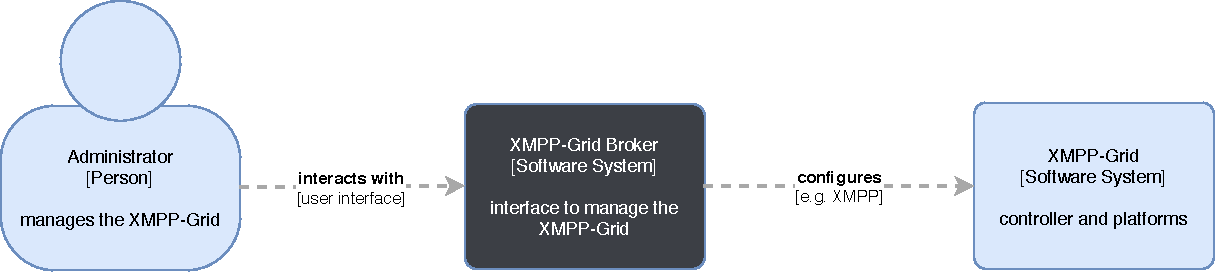
\includegraphics[width=\linewidth]{resources/architecture_context}
\caption[Architecture Context Diagram]{Architecture diagram showing the context of the XMPP grid broker application.}
\label{fig:architecturecontext}
\end{figure}


\subsection{Architectural Style and Platform}

To implement the XMPP grid broker, we evaluated three possible architecture styles:\hfill\\
An XMPP Server Plugin (e.g. extension for the Openfire XMPP server), an implementation with the Jabber Component Protocol~\cite{xep-0114} or an implementation acting as a regular XMPP client ("bot").

We decided to build an XMPP client/bot, because it is not coupled to a specific XMPP server as the Server Plugin and, in contrast to the XMPP Component, supports a strong authentication mechanism with SASL.

The full decision argument is documented in Appendix~\fullref{sec:architectural-decisions}.

\subsubsection{Platform}

The proposed XMPP client might be implemented in three different ways: as rich client application with a command line or graphical interface as illustrated in Figure~\ref{fig:architecturecontainerrichclient}, or in the form of a web application, illustrated in Figure~\ref{fig:architecturecontainerwebapplication} and \ref{fig:architecturecontainerwebproxy}.

\begin{figure}[h]
\centering
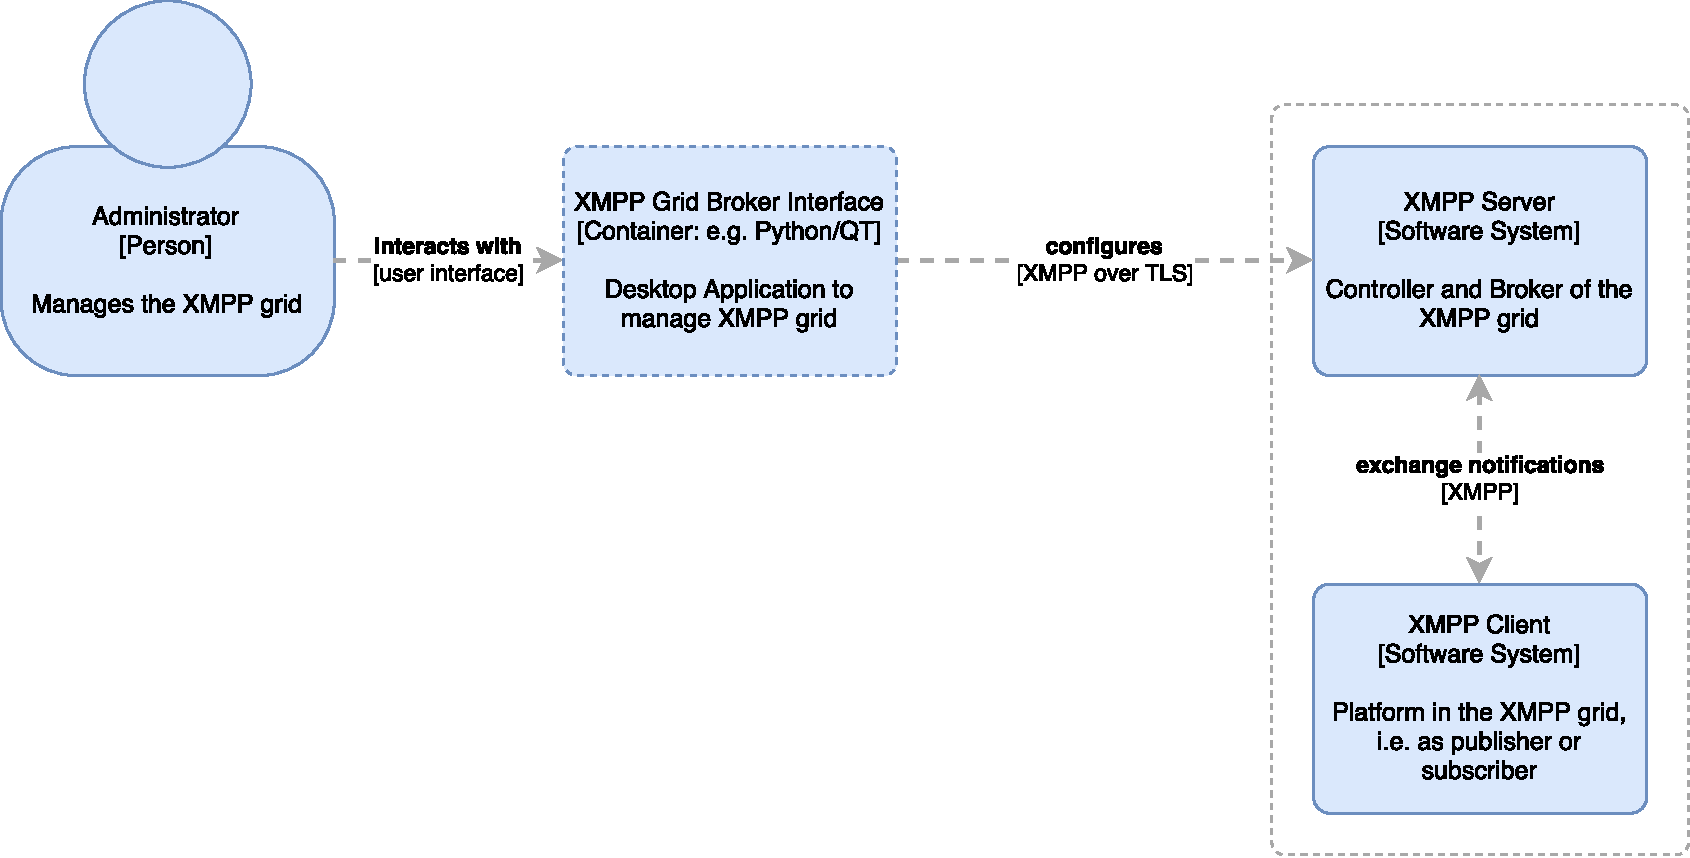
\includegraphics[width=0.7\linewidth]{resources/architecture_container_rich_client}
\caption[Architecture Container Diagram: Rich Client]{Architecture Container Diagram showing a possible rich client architecture.}
\label{fig:architecturecontainerrichclient}
\end{figure}

A web application has the significant advantage to be easily installable, upgradable and has minimal requirements on the user's side (i.e. only requires a web browser to be executed).
Therefore, we decided to implement the XMPP grid broker as web application.

\subsection{Web Application Topology}

To manage the Controller from our interface, we considered the implementation of either directly connecting to the XMPP server over WebSockets~\cite{rfc7395} or HTTP (BOSH~\cite{xep-0124}), or to communicate indirectly with the XMPP server via custom WebAPI Proxy.
These topologies are illustrated in Figure~\ref{fig:architecturecontainerwebapplication} and Figure~\ref{fig:architecturecontainerwebproxy}.

As elaborated in the according design decision (see Appendix~\ref{sec:architectural-decisions}), we decided for the direct connection via WebSockets.
This topology simplifies the implementation and deployment of the application in comparison to a WebAPI Proxy.
Additionally, WebSockets offer stateful TCP-sockets to exchange data with the XMPP server in contrast to BOSH, which uses HTTP long polling to emulate a bidirectional stream~\cite{xep-0124}.

Using the XMPP Service Discovery~\cite{xep-0030}, the XMPP server may be queried for supported features, so that only supported functionality is presented to the application user.

\begin{figure}[h]
\centering
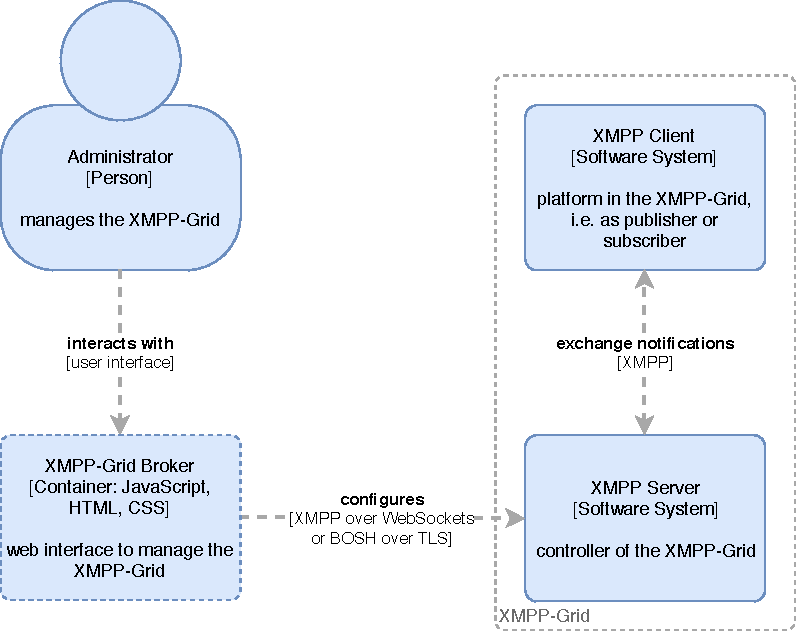
\includegraphics[width=0.7\linewidth]{resources/architecture_container_webapplication}
\caption[Architecture Container Diagram: Web Application]{Architecture Container Diagram showing the web application topology with WebSockets or BOSH.}
\label{fig:architecturecontainerwebapplication}
\end{figure}

\begin{figure}[h]
\centering
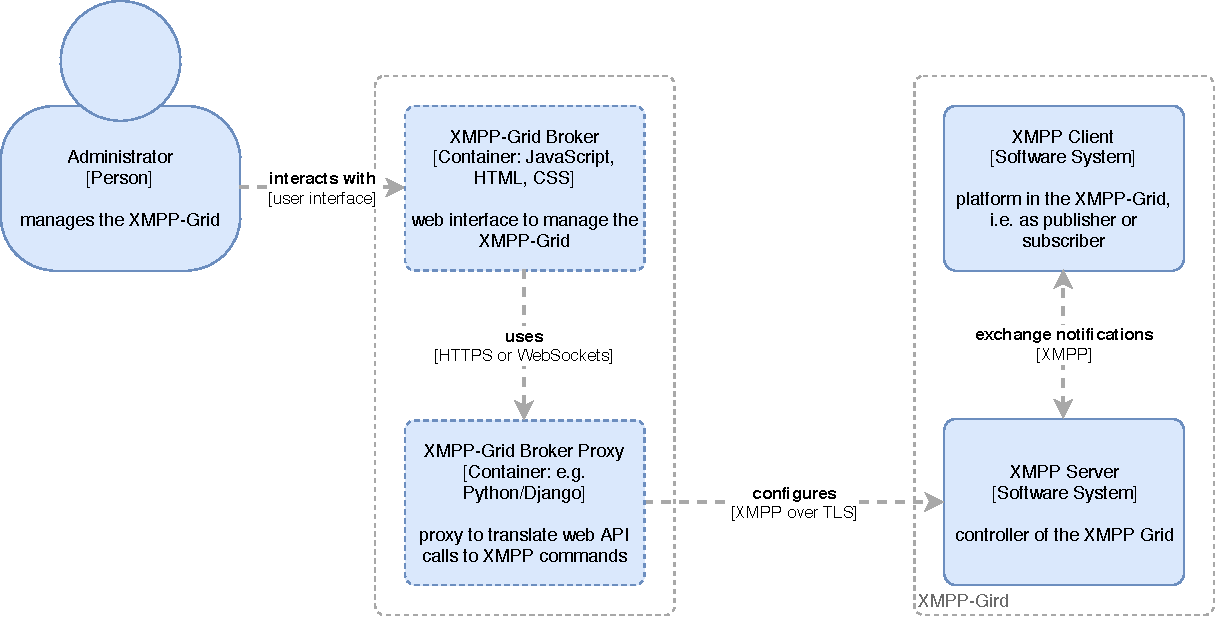
\includegraphics[width=0.7\linewidth]{resources/architecture_container_proxy.pdf}
\caption[Architecture Container Diagram: Web Proxy]{Architecture Container Diagram showing the WebAPI Proxy topology.}
\label{fig:architecturecontainerwebproxy}
\end{figure}


\subsection{Authentication and Connection Security}

XMPP uses SASL as authentication mechanism~\cite{rfc6120}.
To authenticate against the XMPP Grid Controller, we decided to use the SASL EXTERNAL~\cite{rfc4422} mechanism whenever possible to authenticate the client.

We decided against the alternative SASL authentication method, SASL SCRAM~\cite{rfc7677}, that is also recommended by in the XMPP grid draft~\cite{ietf-mile-xmpp-grid-05}.
As described in the corresponding architectural decision (Appendix~\ref{sec:architectural-decisions}), the main reason for SASL EXTERNAL is its higher level of security and and its relatively simple scaling capabilities.

SASL EXTERNAL implies that the authentication takes place on a lower layer than the actual XMPP protocol. In our case, this implies authentication over TLS, i.e.~X.509 end-user certificates as specified in RFC6120~\cite{rfc6120}.


\section{Wireframes}

We created wireframes for most screens to visualise the initial set of user stories.
They helped us to find missing requirements, most notably the support of collections.
All wireframes are listed in Appendix~\fullref{sec:wireframes}.

\section{Security Considerations}\label{sec:security-considerations}

Regarding only the XMPP-Grid Broker application, there are three primary attack vectors:

\begin{description}
    \item[Client-side attacks,] e.g. via web browser, web browser extension or malicious software on the client operating system.
    \item[Web server attacks,] e.g. misconfiguration or insufficient hardening.
    \item[XMPP server attacks,] e.g. misconfiguration or insufficient hardening.
\end{description}

Details on all attack vectors are discussed in the following sections.

\subsection{The XMPP Protocol}

An in-depth security analysis of the XMPP protocol is out of the scope of this thesis.
A detailed discussion of security concerns can be found in the XMPP specification~\cite{rfc6120} and most XEPs~\cite{xep-0060}\cite{xep-0248}.
In this section, we highlight the most crucial security concerns relevant to this thesis.

\subsubsection{Transport Security}

XMPP reuses many established and standardised mechanisms to improve the protocol security.
By layering protocols in a strict manner (XMPP with SASL over TLS over TCP), many attack scenarios such as replaying or eavesdropping are minimised.
The protocol also requires clients and servers to validate the certificates of the other party.~\cite{rfc7590}\cite{rfc6120}

\subsubsection{Protocol}

Since XMPP is based on XML, it inherits some of its security implications.
XMPP prohibits some XML features such as comments and external entity references which mitigate common attacks.~\cite{rfc6120}

The protocol itself cannot mitigate attacks where an attacker gains access to account credentials.
To prevent such corruptions best practices such as storing certificates and passwords securely must be followed.

\subsubsection{PubSub Collection Nodes}

The use of PubSub Collection Nodes~\cite{xep-0248} can leak private data if not configured properly.
Administrators must take great care when configuring collection nodes.
The XMPP-Grid Broker should support Administrators to detect such data leaks.

\subsection{Client Security}

Because the web has many potential security concerns, above all a modern web browser is critical for client security.
Legacy browsers can not provide an adequate level of security.~\cite{firefox-update-security}

Most browser support extension mechanisms which have rather significant capabilities.
The usage of untrusted or uncertified browser extensions is strictly discouraged.~\cite{browser-extension-security}

The same applies to the client operating system and all software installed on clients.

\subsubsection{Authentication and Authorisation}

Regarding authentication and authorisation, the XMPP server does most of the heavy lifting such as storing passwords and validating certificates.
On the client side, the browser does most of that work too (i.e. validating certificates).

The responsibility of our client implementation is to establish a secure channel to the XMPP server and warn the user if a problem occurs during this process (e.g. invalid server certificate).

\subsubsection{Angular Framework}

Using the Angular framework impacts client security significantly.
Angular is built with security in mind and is adopted in the industry in security-relevant environments.
Therefore, Angular receives frequent security updates and is well tested.
By using plain JavaScript, it's unlikely to achieve the same level of security in a reasonable timespan.

On their project website, Angular recommends the following three best practices regarding security~\cite{angular-security}.

\begin{itemize}
    \item Keep current with the latest Angular library releases.
    \item Don't modify your copy of Angular.
    \item Avoid Angular APIs marked in the documentation as ''Security Risk''.
\end{itemize}

We can ensure the later two by making them acceptance criteria.
Keeping current with the latest Angular releases is harder, as our work on this project is limited.
To ensure that future updates can easily be applied we deviate as less as possible from the standard angular setup (e.g. by not ejecting the Webpack configuration\footnote{\url{https://github.com/Angular/Angular-cli/wiki/eject}}).

Keeping Angular up-to-date is of paramount importance as potential vulnerabilities (e.g. XSS) can be exploited if not patched.

\subsubsection{Angular Content Security}

Except for \glspl{persisted-item}, no XMPP content is displayed directly but serves as the basis for rendered HTML components.
To protect against malicious payloads, the received XML messages must be validated before their usage.

\Glspl{persisted-item} can contain an arbitrary content and must therefore be escaped before rendering to prevent Cross-Site Scripting (XSS) attacks.

Angular supports these measures by treating all values (except Angular templates) as untrusted by default.
With regards to the Angular templates, we use the offline template compiler, so that no user-generated data can influence them. To fully utilise the security measures provided by Angular, their APIs must be used at all times instead of direct use of the DOM-APIs.~\cite{angular-security}

Using Content-Security-Policy (CSP) provides additional XSS-protection mechanisms \cite{w3c-csp}.
The XMPP-Grid Broker should document an appropriate CSP, that must be supported in a production environment.

\subsection{Server Security}

\subsubsection{Authentication and Authorisation}

The XMPP server implements most of the authentication and authorisation mechanisms used in a XMPP-Grid Broker implementation, such as storing passwords and validating certificates.

The web server hosting the client application has no active authentication or authorisation responsibility, except to ensure the integrity and authenticity of the application, i.e. by using TLS.

\subsubsection{Web Server}

To minify security concerns on the server side, we decided to keep the server side static (See \fullref{sec:architectural-decisions}).
This allows operators to use any standard web server (e.g. NGINX, Apache, etc.) to serve the client.
Securing such standard web servers is common knowledge for operators and is out of the scope of this analysis.

In addition to these general best practices, we explicitly recommend the following security measures to maximise the client security:

\begin{itemize}
    \item Enable Content Security Policy (CSP)~\cite{w3c-csp}.
    \item Use secure TLS configurations such as secure Cipher Suites, strictly Honor Cipher Order, HSTS, HPKP and OCSP Stapling\footnote{\url{https://wiki.mozilla.org/Security/Server_Side_TLS}}.
\end{itemize}


\subsubsection{XMPP Server}

The XMPP server security depends on the chosen implementation and the application domain.
Discussing XMPP server security in detail is out of the scope of this thesis.
Operators should adhere to the security recommendations of their XMPP server vendor and follow general security best practices as outlined by the XMPP-Grid draft~\cite{ietf-mile-xmpp-grid-05}.

\section{Security Risk Mitigation}

To mitigate the security risks as discussed in Section~\ref{sec:security-considerations}, we implement the measures as described in the following subsections.

\subsection{Development}

\begin{enumerate}
    \item Conduct Code Reviews for all newly added code using GitHub pull requests and a security checklist (See next section)
    \item Conduct an architectural analysis with an industry expert.
    \item Define explicit security requirements in the form of constraints
    \item Automate build and release processes to minimise the time required to patch.
    \item Stay as close to the default Angular setup to simplify further updates
    \item Avoid additional third-party dependencies whenever possible
\end{enumerate}

\subsection{Client Security Checklist}
\begin{itemize}
    \item The latest Angular-version is used
    \item No customizations are made to the Angular version
    \item No direct access to DOM-APIs
    \item APIs marked in the documentation as ``Security Risk'' are \emph{not} used
    \item No usage of any Methods starting with \texttt{bypassSecurityTrust}.
    \item The client is fully Content Security Policy compliant
    \item The client is fully Same Origin Policy (SOP) / Cross-Origin Resource Sharing (CORS) compliant
    \item Only complete templates offline using the offline template compiler.
    \item User input is always escaped using the mechanisms provided by the framework
    \item XMPP-Messages are validated to contain only the specified result-types
\end{itemize}